\documentclass[a4paper]{article}
\usepackage[14pt]{extsizes} % для того чтобы задать нестандартный 14-ый размер шрифта
\usepackage[margin=0.7in]{geometry}
\usepackage{multirow}
\usepackage {graphicx}
\usepackage[utf8x]{inputenc} % указать кодировку русского текста
\usepackage[russian]{babel} % указать, что язык текста - русский
\usepackage{fancyhdr}
\pagestyle{fancy}
\usepackage{graphicx}
\graphicspath{{pictures/}}
\DeclareGraphicsExtensions{.pdf,.png,.jpg}
\usepackage{tocloft}
\renewcommand{\cftsecleader}{\cftdotfill{\cftdotsep}}
\begin{document} 
 \begin{titlepage}
\begin{center}
\hfill \break
Министерство науки и высшего образования Российской Федерации\\
ФЕДЕРАЛЬНОЕ ГОСУДАРСТВЕННОЕ АВТОНОМНОЕ ОБРАЗОВАТЕЛЬНОЕ\\ 
УЧРЕЖДЕНИЕ ВЫСШЕГО ОБРАЗОВАНИЯ\\ 
«МОСКОВСКИЙ ФИЗИКО-ТЕХНИЧЕСКИЙ ИНСТИТУТ\\ 
(НАЦИОНАЛЬНЫЙ ИССЛЕДОВАТЕЛЬСКИЙ УНИВЕРСИТЕТ)»\\
(МФТИ)\\
\hfill \break
\hfill \break
\hfill \break
\hfill \break
\hfill \break
\hfill \break
\hfill \break
\hfill \break
\hfill \break
\hfill \break
\hfill \break
КАФЕДРА ОБЩЕЙ ФИЗИКИ\\
\hfill \break
ВОПРОС ПО ВЫБОРУ\\
ПО ЛАБОРАТОРНОЙ РАБОТЕ 3.7.1\\
\hfill \break
СКИН-ЭФФЕКТ В ПОЛОМ ЦИЛИНДРЕ\\
\end{center}
\hfill \break
\hfill \break
\hfill \break
\hfill \break
\hfill \break
\hfill \break
\hfill \break
\hfill \break
\begin{tabular}{ccc}
Работу выполнила студентка группы Б04-004 & \underline{\hspace{3cm}}& М.В.Шлапак \\\\
\end{tabular}
\hfill \break
\hfill \break
\hfill \break
\hfill \break
\hfill \break
\hfill \break
\hfill \break
\begin{center} Долгопрудный 2021 \end{center}
\end{titlepage}
\small
\fancyhead[L] {Скин-эффект в полом цилиндре}
\tableofcontents    
\newpage
\section{Цель работы}
\begin{enumerate}
    \item Изучить явление скин-эффекта.
    \item Исследовать проникновение переменного магнитного поля в медный полый цилиндр.
\end{enumerate}
\section{Приборы и материалы}
В работе используются генератор звуковой частоты, соленоид, намотанный на полый цилиндрический каркас из диэлектрика, медный кран в виде трубки, измерительная катушка, амперметр, вольтметр, осциллограф.
\section{Теоретические сведения}
\subsection{Электромагнитные волны}
Система уравнений Максвелла являются фундаментом современной электродинамики сплошных сред. \\
$$1. \oint{\overrightarrow{D}\overrightarrow{dS}} = 4\pi q \; \;\;\;\; \mathrm{div} \overrightarrow{D} = 4\pi\rho \; \;   \; \;\;\; q = \int{\rho dV} \eqno(3.1.1)$$ 
$$2. \oint{\overrightarrow{B}d\overrightarrow{S}} = 0 \; \; \; \; \; \; \; \; \; \mathrm{div} \overrightarrow{B} = 0 \eqno(3.1.2)$$
$$3. \oint{\overrightarrow{E}d\overrightarrow{l}} = - \int{\frac{\partial \overrightarrow{B}}{\partial t}d\overrightarrow{S}} \; \; \mathrm{rot} \overrightarrow{H} = \overrightarrow{j} + \frac{\partial \overrightarrow{D}}{\partial t} \eqno (3.1.3)$$
$$4. \oint{\overrightarrow{H}d\overrightarrow{l}} = \int{\overrightarrow{j}d\overrightarrow{S}} + \int{\frac{\partial \overrightarrow{D}}{\partial t}d\overrightarrow{S}} \; \; \mathrm{rot}\overrightarrow{H} = \overrightarrow{j} + \frac{\partial \overrightarrow{D}}{\partial t} \eqno(3.1.4)$$

Одним из важнейших следствий теории Максвелла является возможность существования электромагнитных полей в виде волн, способных распространяться независимо от их источников (зарядов и токов). Положим в уравнениях Максвелла $\rho = 0$ и $\overrightarrow{j} = 0$ и воспользуемся материальными уравнениями. Последнее уравнение Максвелла примет вид:\\
$$\frac{1}{\mu \mu_{0}}\mathrm{rot} \overrightarrow{B} = \varepsilon \varepsilon_{0} \frac{\partial \overrightarrow{E}}{\partial t}$$
Продифференцируем обе его части по времени и подставим закон электромагнитной индукции (уравнение 3):\\
$$\mathrm{rot} \; \mathrm{rot} \overrightarrow{E} = - \varepsilon \varepsilon_{0} \mu \mu_{0} \frac{\partial^2 \overrightarrow{E}}{\partial t^2}$$
Далее воспользуемся известной формулой из векторного анализа:\\
$$\mathrm{rot} \; \mathrm{rot} \overrightarrow{E} = \mathrm{grad} \; \mathrm{div} \overrightarrow{E} - \nabla^2 \overrightarrow{E}$$
Учитывая, что в отсутствие зарядов $\mathrm{div} \overrightarrow{E} = 0$, получим окончательно:\\
$$\nabla^2 \overrightarrow{E} = \frac{1}{v^2}\frac{\partial^2 \overrightarrow{E}}{\partial t^2} \eqno(3.1.8)$$
где введена величина, имеющая размерность скорости,
$$v = \frac{1}{\sqrt{- \varepsilon \varepsilon_{0} \mu \mu_{0}}} = \frac{c}{\sqrt{\varepsilon \mu}} \eqno(3.1.9)$$
Уравнение (предпоследнее) называется \em волновым \em. Уравнению такого же вида подчиняются и сотальные характеристики поля \overrightarrow{D}, \overrightarrow{B}, \overrightarrow{H}. Оно описывает распространение элеткромагнитных волн в среде со скоростью $v$, определяемой соотношением выше. Факт распространения электромагнитных полей независимо от создавших их зарядов и токов впервые был экспериментально подтвержден Герцем в 1887 году. \\
\subsection{Волны в безграничной среде}
Простейшим частным решением волнового уравнения (3.1.8) в безграничном пространстве является плоская волна:
$$\overrightarrow{E}(t, \overrightarrow{r}) = \overrightarrow{E_0}\sin{(\omega t - \overrightarrow{k}\cdot \overrightarrow{r})} \eqno(3.2.1)$$
Эта волна распространяется вдоль волнового вектора $\overrightarrow{k} = (k_x, k_y, k_z)$. Его модуль связан с длиной волны соотношением $\lambda = 2\pi/k$.\\
Подставив (3.2.1) в (3.1.8) нетрудно получить условие, которому должны удовлетворять компоненты волнового вектора плоской волны:
$$k^2_x + k^2_y + k^2_z = \frac{\omega^2}{v^2} \eqno(3.2.2)$$
Это условие называют \em дисперсионным соотношением \em для плоских электромагнитных волн. Отсюда, в частности, следует, что $v = c/ \sqrt{\varepsilon \mu}$ - фазовая скорость элеткромагнитной волны в свободном пространстве:
$$v_f = \frac{\omega}{k} = v$$
Поскольку волновое уравнение линейно, его общее решение в свободном пространстве является линейной комбинацией плоских волн, удовлетворяющих дисперсионному соотношению. \\
\subsection{Квазистационарное приближение}
Рассмотрим переменные электромагнитные поля в хорошо проводящих средах. Если характерная чатсота изменения поля достаточно мала, а проводимость среды, наоборот, велика, то можно пренебречь током смещения по сравнению с токами проводимости $j$. Электрическое поле и ток в среде будем считать связанными законом Ома (3.1.7). Уравнение (3.1.4) без тока смещения представляет собой закон Ампера для постоянного поля. В дифференциальной форме:
$$\mathrm{rot} \overrightarrow{H} = \sigma \overrightarrow{E} \eqno(3.3.1)$$
Кроме того учтём, что переменное магнитное поле вызывает вихревое электрическое поле согласно закону электромагнитной индукции (2.1.3). Пренебрежение током смещения в уравнениях поля формально соответствует бесконечной скорости распространения элеткромагнитных волн (вне проводника). Такое приближение принято называть \em квазистационарным.\em \\
Выразим уравнения динамики электромагнитных полей в рассматриваемом приближении.
\subsection{Скин-эффект}
Рассмотрим квазистационарное поле внутри проводящей среды в простейшем плоском случае. Пусть вектор $\overrightarrow{E}$ направлен всюду вдоль оси y и зависит только от координаты x, то есть $E_x = E_z = 0$, $E_y = E_y(x,t)$. Тогда уравнение для электрического поля будет иметь вид:
$$\frac{\partial^2 E_y}{\partial x^2} = \sigma \mu \mu_0 \frac{\partial E_y}{\partial t} \eqno(3.4.1)$$
Пусть полупространство x>0 заполнено проводящей средой с проводимостью $\sigma$, а на границе x = 0 задано электрическое поле, изменяющееся по гармоническому закону $E_y = E_0e^{i\omega t}$. Будем искать решение уравнения (3.4.1) также в виде гармонической функции:
$$E_y(x,t) = E(x)e^{i\omega t}$$
где $E(x)$ - комплексная амплитуда колебаний поля, зависящая от координаты x. После подстановки в (3.4.1) получим уравнение на функцию $E(x)$:
$$\frac{d^2E}{dx^2} = i\omega \sigma \mu \mu_0 E \eqno(3.4.2)$$
Как известно из теории линейных дифференциальных уравнений, решение (3.4.2) нужно искать в виде: $$E(x) = E_0e^{\alpha x} \eqno(3.4.3)$$, где $\alpha$ - комплексная константа. Подставляя (3.4.3) в (3.4.2) получаем, что уравнение имеет нетривиальные решения такого вида при
$$\alpha^2 = i \omega \sigma \mu \mu_0 \eqno(3.4.4)$$
Отсюда, поскольку $\sqrt{i} = \pm \frac{1+i}{\sqrt{2}}$,
$$\alpha = \pm \frac{1+i}{\sqrt{2}} \sqrt{\omega \sigma \mu \mu_0}$$
Для полубесконечной среды (z>0) физический смысл имеет только решение со знаком минус, соответствующее стремлению к нулю амплитуды поля при стремлении к бесконечности z. окончательное решение уравнения (3.4.1) для нашего случая:
$$E_y(x, t) = E_0e^{-x/\delta}e^{i(\omega t - x/\delta)} \eqno(3.4.5)$$
где 
$$\delta = \sqrt{\frac{2}{\omega \sigma \mu \mu_0}} = \sqrt{\frac{2D}{\omega}} \eqno(3.4.6)$$
Из полученного решения (3.4.5) видно, что амплитуда переменного
электрического поля с частотой $\omega$ убывает вглубь проводника по экспоненциальному закону. Такой закон спадания характеризуется расстоянием $\delta$, на котором амплитуда поля уменьшается в 𝑒 раз.\\ Это расстояние называют \em глубиной проникновения \em поля или \em скиновой \em длиной. Как показывает (3.4.6), с ростом частоты $\omega$ электрическое поле всё более «вытесняется» к поверхности проводника. Это явление называется
\em скин-эффектом \em (от англ. skin — кожа).\\
\\
Поскольку уравнение для магнитного поля  совершенно аналогично уравнению для напряжённости электрического поля, то очевидно, что $H_z(x)$ убывает вглубь проводника точно по такому же закону,
как и $E_y(x)$. Если поместить проводящий образец в переменное внешнее магнитное поле (например, металлический сердечник в катушку), оно будет проникать в проводник на глубину скин-слоя $\delta$, индуцируя в нём переменное электрическое поле, которое в свою очередь вызывает появление токов (\em токи Фуко \em). Возникновение токов Фуко сопровождается по закону Джоуля–Ленца диссипацией энергии поля с превращением её в тепло.\\
Обобщение на неплоский случай представляет собой существенно более сложную задачу, имеющую в общем случае лишь численное решение.
Однако выражение для характерной глубины проникновения поля (3.4.6)
остаётся верным по порядку величины для любой формы проводника.\\
\subsection{Скин-эффект в полом цилиндре}
Пусть цилиндр достаточно длинный,
так что в нём можно пренебречь краевыми эффектами. В этом приближении
магнитное поле H всюду направлено по
оси системы (ось 𝑧), а вихревое электрическое поле E будет всюду перпендикулярно радиусу, то есть линии поля образуют соосные окружности. Все
величины будем считать колеблющимися по гармоническому закону с некоторой
частотой $\omega$, задаваемой частотой колебания тока в соленоиде. Тогда для ненулевых компонент поля можно записать
$$H_z = H(r)e^{i\omega t} \; \; \; \; E_{\varphi} = E(r)e^{i \omega t}$$
где H(r) и E(r) — комплексные амплитуды колебаний соответствующих
полей, зависящие только от расстояния 𝑟 до оси системы. Заметим, что
на границе цилиндра должны быть непрерывны касательные к поверхности компоненты как E, так и B, поэтому функции E(r) и H(r) непрерывны во всей исследуемой области.\\
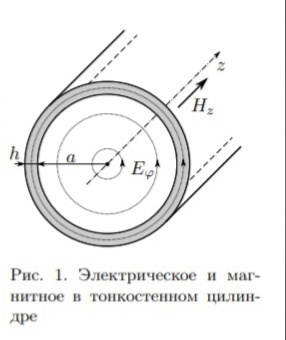
\includegraphics[width=5cm]{g7}\\

\section{Ход работы}
\subsection{Экспериментальная установка}
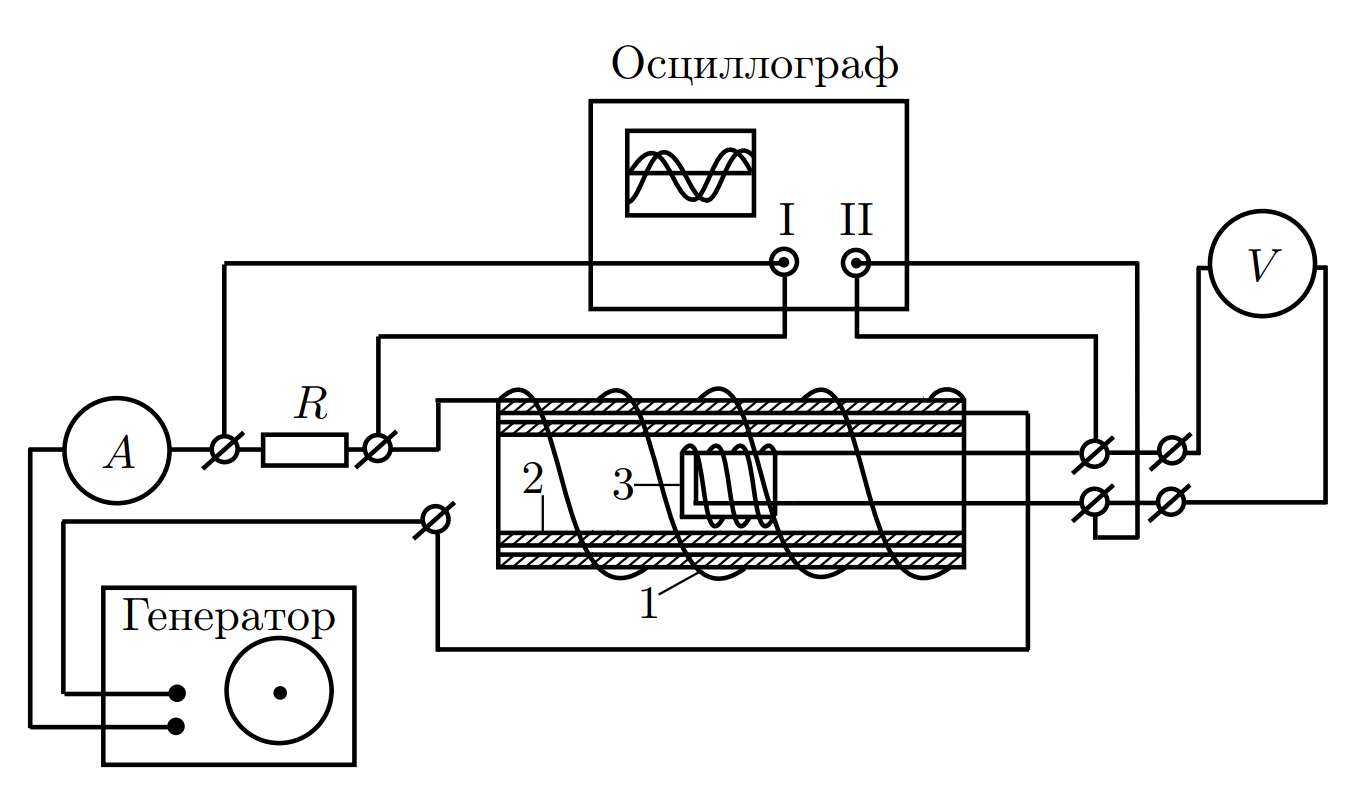
\includegraphics[width=15cm]{g1}\\
Переменное магнитное поле создается с помощью соленоида, намотанного на полый цилиндрический каркас 1 из поливинилхлорида, который подключается к генератору звуковой частоты. Внутри соленоида расположен медный цилиндрический экран 2. Для измерения магнитного поля внутри экрана используется измерительная катушка 3. Действующее значение переменного тока в цепи соленоида измеряется амперметром А, ад ействующее значение напряжения на измерительной катушке измеряет вольтметр V. Для измерения сдвига фаз между током в цепи соленоида и напряжением на измерительной катушке используется двухканальный осциллограф. На вход одного канала подается напряжение с резистора R, которое пропорционально току, а на вход второго канала - напряжение с измерительной катушки. \\
\subsection{Измерение отношения амплитуд магнитного поля внутри и вне экрана}
С помощью вольтметра V измеряется действующее значение ЭДС индукции, которая возникает в измерительной катушке, находящейся в переменном магнитном поле $H_1e^{iwt}$. Комплексная амплитуда ЭДС индукции в измерительной катушке равна:
$$U = -SN\frac{dB_1(t)}{dt} = -iw\mu_{0}SNH_1e^{iwt}$$
где $SN$ - произведение площади витка на число витков измерительной катушки. Показания вольтметра, измеряющего это напряжение:
$$ U = \frac{SNw}{\sqrt{2}}\mu_{0}|H_1|$$
Видно, что модуль амплитуды магнитного поля внутри экрана $|H_1|$ пропорционален U и обратно пропорционален чатсоте сигнала $\nu = \omega/2\pi$:
$$|H_1| \propto \frac{U}{\nu}$$
При этом поле вне экрана $|H_0|$ пропорционально току I в цепи соленоида, измеряемому амперметром А:
$$|H_0| \propto I$$
Следловательно, 
$$\frac{|H_1|}{|H_0|} = const \cdot \frac{U}{\nu I}$$
Таким образом, отношение амплитуд магнитных полей снаружи и вне экрана (коэффициент ослабления) может быть измерено по отношению $U/\nu I$ при разных частотах. Неизвестная константа в соотношении выше может быть определена по измерениям при малых частотах $\nu \rightarrow 0$, когда согласно уравнению из теории $|H_1|/|H_0| \rightarrow 1$.\\
\subsection{Определение проводимости материала экрана}
В установке в качестве экрана используется медная труба промышленного производства. Технология изготовления труб оказывает заметное влияние на электропроводимость. Из-за наличия примесей проводимость меди нашей трубы отличается от табличного значения (в меньшую сторону). Для определения $\sigma$ нашего экрана предлагается использовать частотную зависимость фазового сдвига между магнитными полями внутри и вне экрана при высоких чатсотах. Как видно из выражения, в области больших частот $\omega >> 1/(h^2\sigma \mu_0$ зависимость $\psi(\sqrt{\omega})$ аппроксимируется прямой, проходящей через точку $\psi(0) = \pi/4$. По наклону этой прямой можно вычислить проводимость материала экрана. \\
Заметим, что на схеме экспериментальной установки на входной канал 2 осциллографа подается сигнал с измерительной катушки, который пропорционален не полю внутри экрана, а его производной по времени, а это означает, что появляется дополнительный сдвиг по фазе на $\pi/2$. Поэтому измеренный по экрану осциллографа сдвиг по фазе между двумя синусоидами будет на $\pi/2$ больше фазового сдвига между магнитными полями вне и внутри экрана.\\
\subsection{Выполнение работы}
1) Параметры установки:\\
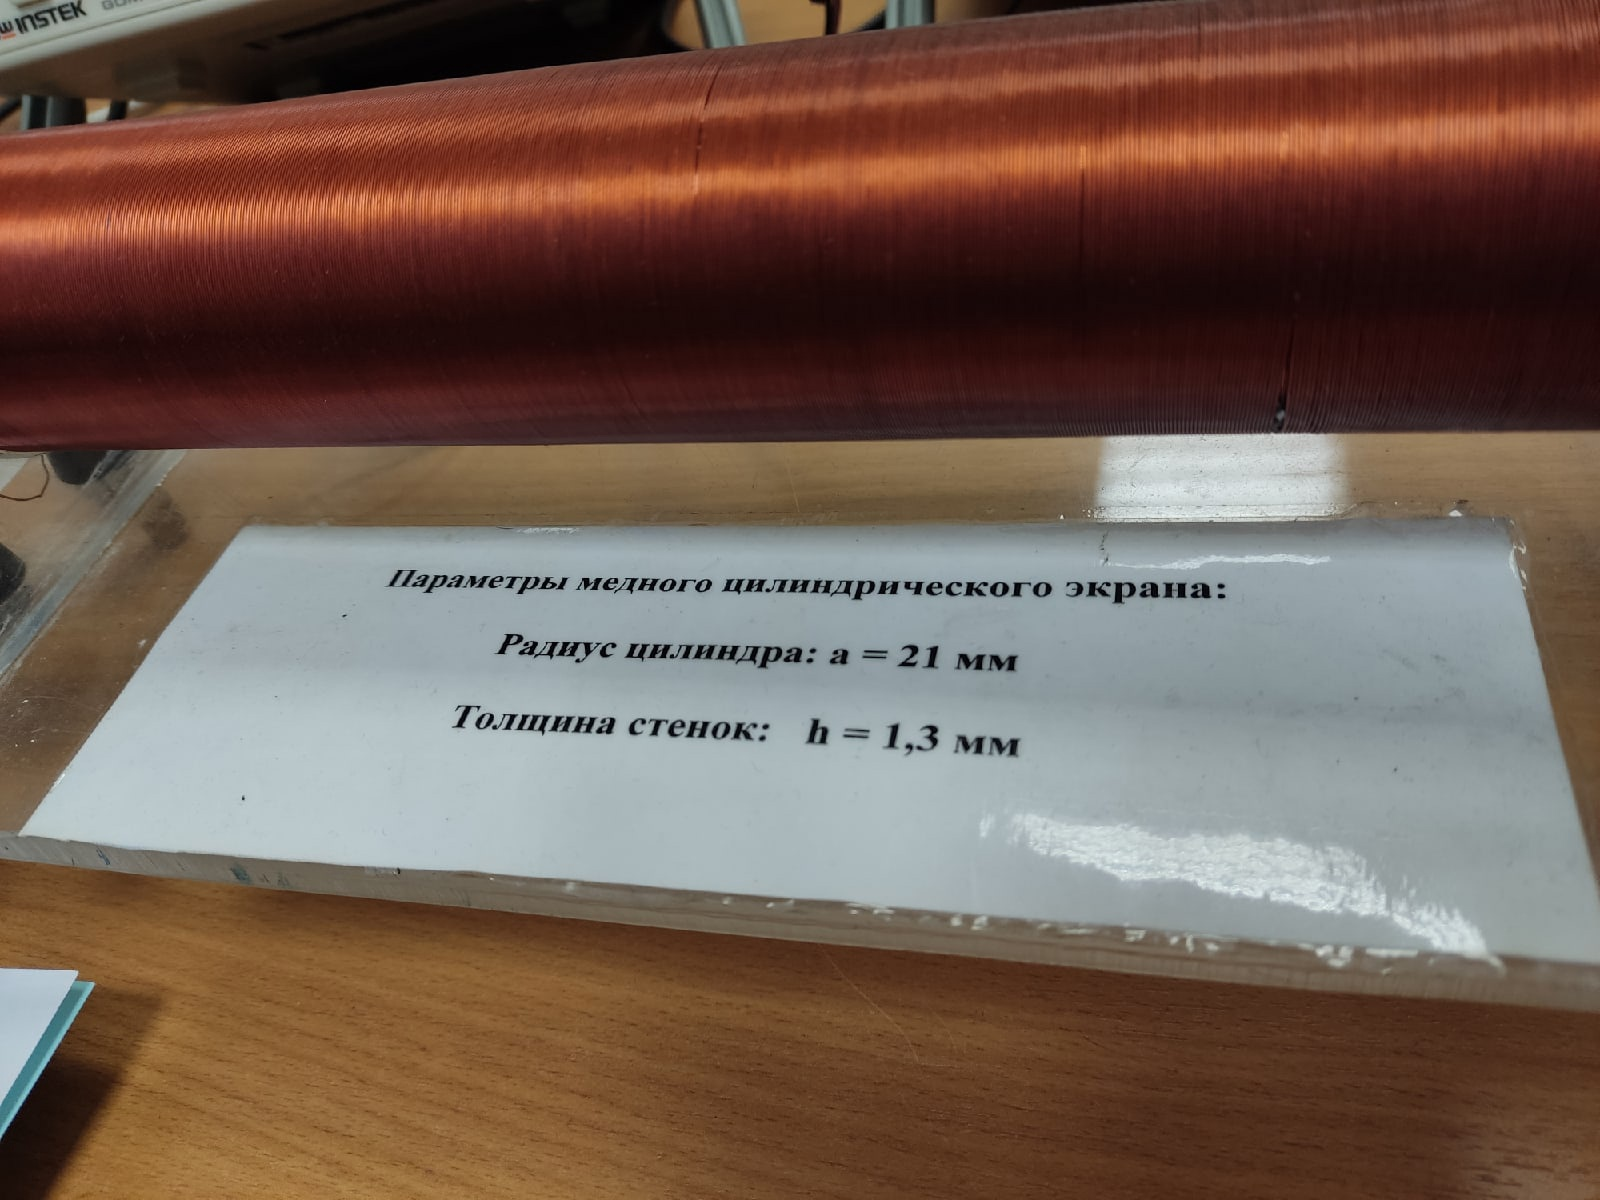
\includegraphics[width=10cm]{g2}\\
2)  В области низких частот 20 - 100 Гц (через $\triangle f = 5$ Гц) снимем зависимость $\xi = U/\nu I$ от частоты $\nu$.\\
Заметим, что при маленькой частоте показания амперметра очень скачут из-за чувствительности, поэтому берем большую погрешность.\\
\begin{tabular}{|l|l|l|l|}\\
\hline
$f$, Гц & $U$, В, $\sigma_{U} = 0,0001$ В & $I$, mA, $\sigma_I = 2,0$ mA & $\sigma_{f}$, Гц\\ \hline
20 & 0,0119 & 53,3 & 0,25 \\ \hline
25 & 0,0145 & 53,5 & 0,25 \\ \hline
30 & 0,0179 & 53,6 & 0,5 \\ \hline
35 & 0,0207 & 53,7 & 0,5 \\ \hline
40 & 0,0234 & 53,6 & 0,5 \\ \hline
45 & 0,0263 & 53,7 & 0,5 \\ \hline
50 & 0,0290 & 54,8 & 0,5 \\ \hline
55 & 0,0322 & 54,0 & 0,5 \\ \hline
60 & 0,0346 & 54,2 & 0,5 \\ \hline
65 & 0,037 & 54,1 & 1 \\ \hline
70 & 0,0398 & 53,9 & 1\\ \hline
75 & 0,0425 & 53,9 & 1\\ \hline
80 & 0,0450 & 53,9 & 1 \\ \hline
85 & 0,0477 & 53,8 & 1\\ \hline
90 & 0,0500 & 53,8 & 1 \\ \hline
95 & 0,0529 & 53,8 & 1\\ \hline
100 & 0,0548 & 53,7 & 1 \\ \hline
\end{tabular}\\
По результатам измерений построим график в координатах $1/\xi^2 = f(f^2)$.\\
\\
Рассчитаем погрешности:\\
$$ (\frac{\sigma_{\xi}}{\xi})^2 = (\frac{\sigma_{U}}{U})^2 + (\frac{\sigma_{f}}{f})^2 + (\frac{\sigma_{I}}{I})^2 \approx (\frac{0,0001}{0,034})^2 + (\frac{0,7}{60})^2 + (\frac{2,0}{53,8})^2 \approx 0,00152 $$ 
Тогда: $\sigma_{\xi} \approx 0,0004 $\\
Тогда погрешность вычисления $1/\xi^2$ равна:
$$\sigma_{1/\xi^2} = 2\sigma_{\xi}/\xi^3 \approx 653 $$
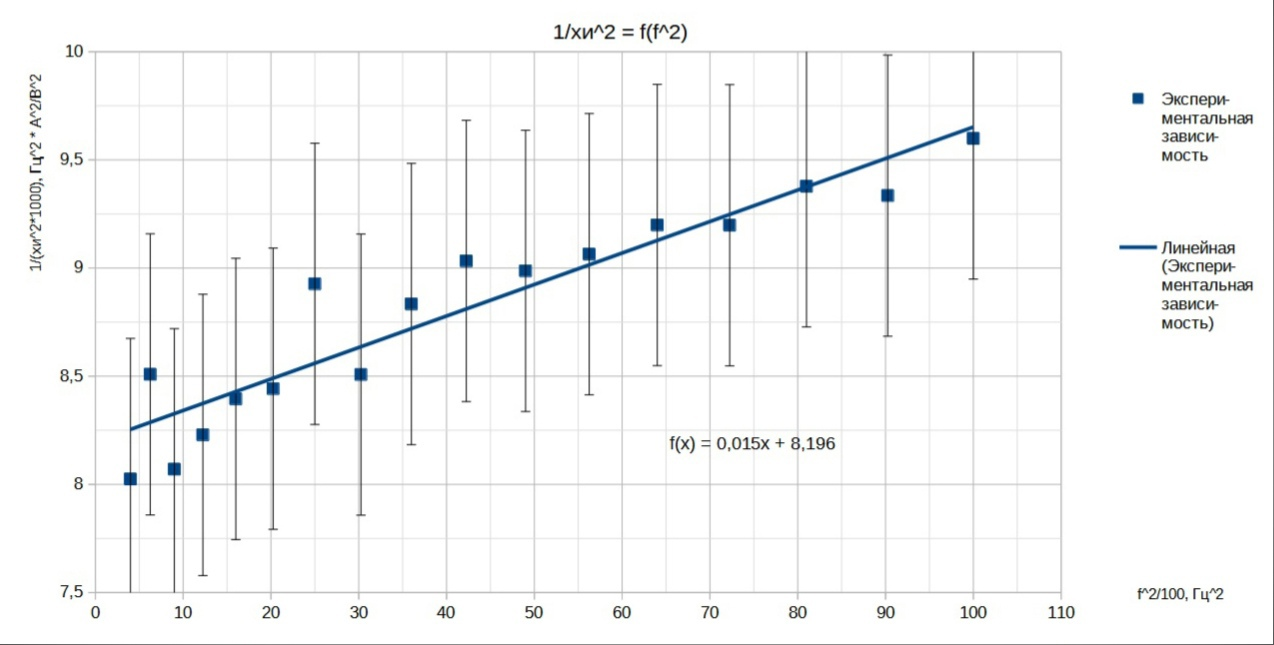
\includegraphics[width=19cm]{g3}\\
Апрроксимировав полученную зависимость прямой, находим её уравнение по МНК:\\
 \fbox{$f(x) = 0,015x + 8,196$}.\\
Эта прямая выражает линейную зависимость:
$$\frac{1}{\xi^2} = \frac{1 + (ah/\delta)^2}{\xi^2_0} = \frac{1 + (ah\pi f \sigma \mu \mu_{0})^2}{\xi^2_0}$$
$$ \xi = \frac{|H_1|}{|H_0|}\xi_0$$
Экстраполируя полученную зависимость к точке $f = 0$, соответствующей $|H_1|/|H_0| = 1$ (числитель равен 1), можем найти постоянную $\xi_0$ (справедливо при малых частотах, когда толщина скин-слоя не превосходит толщину цилиндра):
$$\frac{1}{\xi^2} = \frac{1 + (ah/\delta)^2}{\xi^2_0} = /f = 0/ = \frac{1}{\xi^2_0}$$
Получаем:
$$f(x = 0) = 0,015\cdot 10 \cdot 0 + 8,196 \cdot 1000 = 8196 \; \; => \xi_0 \approx 0,011$$
3) Исследуем зависимость величины фазового сдвига $\triangle \psi$ и $\xi$  в диапазоне 100 - 30 000 Гц и изобразим на графике в координатах $\triangle \psi$ и $\sqrt{f}$.\\
\\
\begin{tabular}{|l|l|l|l|l|l|l|} \hline
f, Гц & U, B  & I, mA  & f, Гц & Хи*1000000 & Сдвиг — Pi/2 & sqrt(f) \\ \hline
100   & 0,05         & 53,69       & 100   & 8,94       & 0,39         & 10,00   \\ \hline
500   & 0,14         & 52,95       & 500   & 5,27       & 1,14         & 22,36   \\ \hline
1000  & 0,16         & 53,88       & 1000  & 2,88       & 1,46         & 31,62   \\ \hline
2000  & 0,16         & 54,43       & 2000  & 1,47       & 1,57         & 44,72   \\ \hline
3000  & 0,16         & 54,03       & 3000  & 0,99       & 1,74         & 54,77   \\ \hline
4000  & 0,16         & 53,63       & 4000  & 0,74       & 2,02         & 63,25   \\ \hline 
5000  & 0,16         & 53,12       & 5000  & 0,59       & 1,71         & 70,71   \\ \hline
6000  & 0,16         & 52,57       & 6000  & 0,49       & 1,90         & 77,46   \\ \hline
7000  & 0,15         & 51,88       & 7000  & 0,42       & 1,96         & 83,67   \\ \hline
8000  & 0,15         & 51,13       & 8000  & 0,37       & 2,02         & 89,44   \\ \hline 
9000  & 0,15         & 50,30       & 9000  & 0,33       & 2,36         & 94,87   \\ \hline
10000 & 0,15         & 49,32       & 10000 & 0,30       & 2,16         & 100,00  \\ \hline
12000 & 0,14         & 47,25       & 12000 & 0,25       & 2,49         & 109,54  \\ \hline 
14000 & 0,13         & 44,62       & 14000 & 0,22       & 2,51         & 118,32  \\ \hline
16000 & 0,13         & 41,60       & 16000 & 0,19       & 2,62         & 126,49  \\ \hline
18000 & 0,12         & 38,80       & 18000 & 0,18       & 2,75         & 134,16  \\ \hline
20000 & 0,13         & 36,20       & 20000 & 0,17       & 3,08         & 141,42  \\ \hline
22000 & 0,12         & 32,04       & 22000 & 0,17       & 3,20         & 148,32  \\ \hline
24000 & 0,11         & 27,18       & 24000 & 0,17       & 3,21         & 154,92  \\ \hline
26000 & 0,11         & 22,10       & 26000 & 0,19       & 3,14         & 161,25  \\ \hline
28000 & 0,10         & 16,50       & 28000 & 0,22       & 3,45         & 167,33  \\ \hline
30000 & 0,10         & 10,90       & 30000 & 0,29       & 3,55         & 173,21 \\ \hline
\end{tabular}
\\
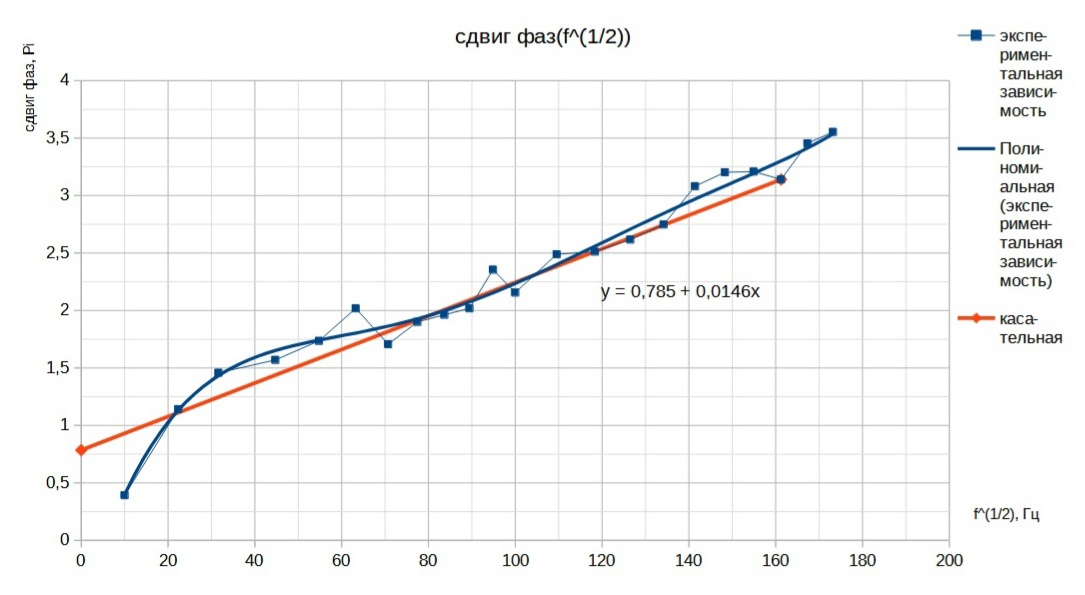
\includegraphics[width=18cm]{g4}\\
Через точку $\triangle \psi = \pi /4$ при $f = 0$ проведем прямую, которая будет пересекаться экспериментальной кривой при больших частотах. По наклону этой прямой вычислим значение проводимости материала экрана и сравним её с табличными результатами для меди. \\
Поле внутри цилиндра запаздывает по фазе на:
$$\psi = \frac{\pi}{4} + h\sqrt{\pi f \sigma \mu_0}$$
Уравнение касательной к графику: $y = \psi(0) + h\sqrt{\pi \sigma \mu_0}x $
Таким образом $k = h\sqrt{\pi \sigma \mu_0} \; \; \; => \sqrt{\sigma} = \frac{k}{h\sqrt{\pi \mu_0}}$\\
$$\sigma = \frac{0,0146^2}{1,3^2 \cdot 10^{-6} \cdot 3,14 \cdot 4 \cdot 3,14 \cdot 10^{-7}} \approx 3,2 \cdot 10^7 $$
Таким образом, экспериментально получили, что проводимость меди равна $3,2 \cdot 10^7$ См/м. В то время как табличное значение для проводимости меди: $5 \cdot 10^7$ См/м.\\
Таким образом, погрешность эксперимента составила $36 \%$. \\
Самое главное, мы совпали по порядку величины, а такая большая погрешность есть следствие не очень точной аппроксимации и не такого большого количесвта точек для последней зависимости.\\
\\
4) Используя вычисленный в пункте два коэффициент $\xi_0$, рассчитаем экспериментальные значения коэффициентов ослабления поля $|H_1|/|H_0|$ для всех измерений пунктов 2 и 3. Изобразим результаты на графике в зависимости от $\sqrt{f}$. \\
$$ \frac{|H_1|}{H_0} = \frac{\xi}{\xi_0}$$
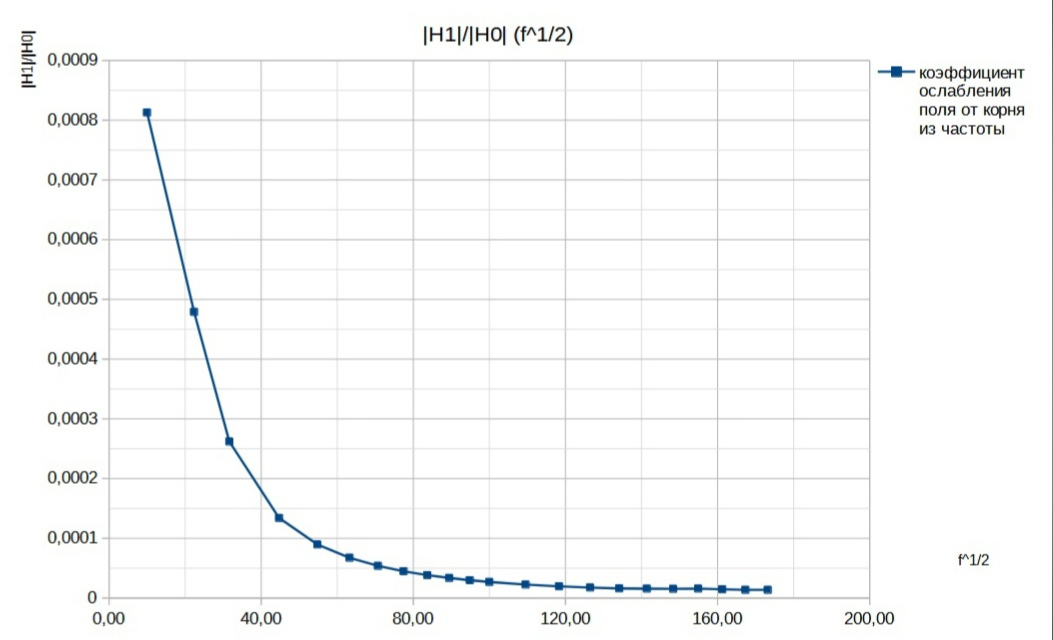
\includegraphics[width=18cm]{g5}\\
Как видно из графика, коэффициент ослабления с увеличением частоты уменьшается, таким образом при больших частотах поле внутри цилиндра очень сильно выталкивается наружу и очень мало по сравнению с внешним полем.\\
5) Воспользовавшись найденным значением $\sigma$, вычислим глубину проникновения поля $\delta$ при двух частотах: 50 Гц и 100 000 Гц.\\
$$\delta = \sqrt{\frac{2}{\omega \sigma \mu \mu_0}} \; \; \;\delta = \sqrt{\frac{1}{ 3,14 \cdot f \cdot \sigma \cdot 4\cdot 3,14 \cdot 1,25 \cdot 10^{1}}}$$
Тогда:\\
$\delta_{50} \approx 1,1$ см\\
$\delta_{100000} \approx 0,3$ мм\\
Эти результаты неплохо сходятся с табличными.\\
\section{Вывод}
1. В результате данной работы было изучено явление скин-эффекта на примере медного полого цилиндра. \\
2. Действительно, опытным путем была получена зависимость коэффициента ослабления магнитного поля внутри цилиндра по отношению к полю снаружи: мы убедились, что магнитное поле внутри очень мало по сравнению с внешним. В ходе опытов также была рассчитана проводимость меди, отклонение экспериментального результата с табличным составило $36 \%$, а также глубина скин-эффекта для двух значений частоты: 50 Гц и 100 кГц. Таким образом, экспериментально подтверждено высказывание о том, что электрическое поле вытесняется к поверхности проводника с ростом частоты. \\
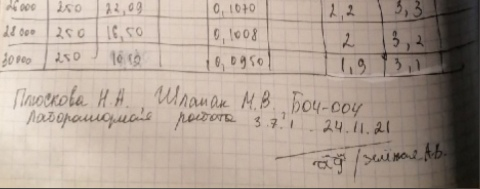
\includegraphics[width=5cm]{g8}\\
\end{document}